\chapter{Konvergence trajektorií}
Jak již bylo naznačeno v úvodní kapitole, v některých případech používáme ke
zlepšení energie aktuální trajektorie backtracking. Nicméně implementovat
backtracking trajektorii až úplně zpět k ústí tunelu by bylo velice nákladné
a neefektivní, proto chceme nějakým způsobem backtracking napojit na již
spočítanou trajektorii, čímž si často můžeme ušetřit značné množství práce.
Uvažme tedy, že máme pozici backtracking trajektorie $ \tilde{\lambda}^i $
na řezu $ \theta_i $ a pozici dopředné trajektorie $ \lambda^i $ na tomtéž řezu.
Nejjednodušším přístupem v takové situaci je zkontrolovat, zda platí
$ \tilde{\lambda}^i \in \Delta \lambda^i $. Tuto kontrolu můžeme provádět v každé
iteraci backtrackingu neboť při ní stačí lineárně projít všechny atomy ligandu
a zkontrolovat jejich vzdálenosti oproti ligandu dopředné trajektorie. Ligandy
navíc typicky mívají velmi malý počet atomů, takže se skutečně jedná o nenáročný
výpočet. Tento přístup bude fungovat ve chvíli, kdy molekula ligandu po opuštění
úzkého hrdla zkonverguje do původní konformace, kterou zaujímá ligand v dopředné
trajektorii, k čemuž dojde zejména v situaci, kdy existuje lokální eneretické
minimum, do kterého se z backtracking konformace můžeme dostat gradientním sestupem.
Této situaci budeme říkat \textit{jednoduchá konvergence}.

\begin{figure}[ht]
\centering
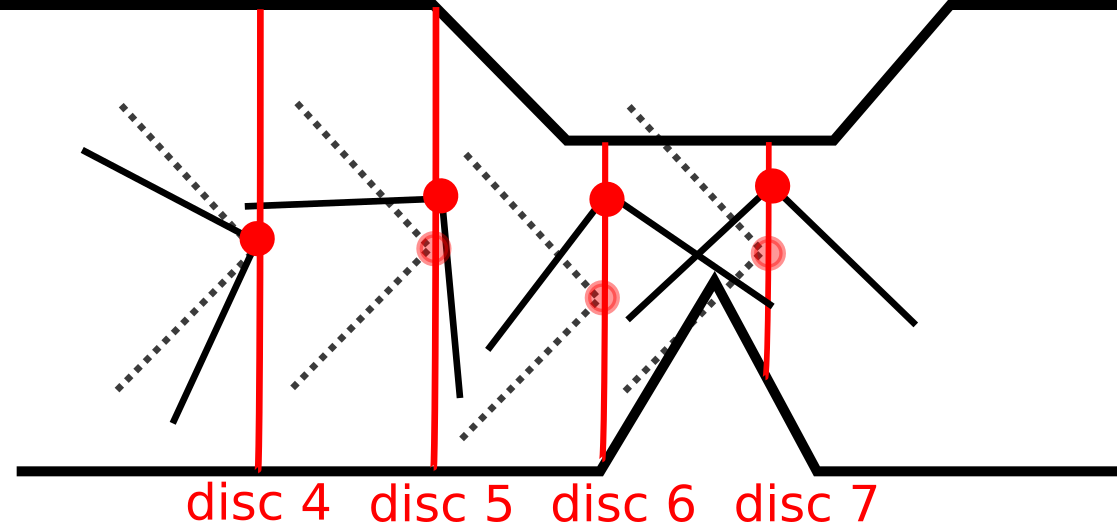
\includegraphics[width=.5\hsize]{img/backtracking_simple.png}
\caption{Jednoduchá konvergence. Dopředná trajektorie je vyznačena tečkovaně,
backtracking plnou čarou.
}
\label{fig:simple_convergence}
\end{figure}


Příklad takové situace můžeme vidět na obrázku č. \ref{fig:simple_convergence}.
Při dopředném pohybu jsme uvázli v úzkém hrdle, ze kterého jsme s vhodnější
konformací spustili backtracking, který po několika iteracích na disku č. 4
samovolně zkonvergoval do pozice, téměř identické s pozicí dopředné trajektorie.
V tuto chvíli by byl backtracking ukončen a dále bychom pokračovali z disku č. 7.

Jednoduchá konvergence může dobu výpočtu zkrátit, nicméně v praxi se často stává,
že ligand při backtrackingu zkonverguje do konformace, které je velmi podobná
konformaci dopředné trajektorie, ale liší se například rotací. Obě pozice tak
mohou mít velice podobnou energii, ale z mělkého lokálního minima se autonomě
nedostanou a backtracking by mohl dospět až k ústí tunelu.
